%! TeX program = lualatex
\mode*
\section{Introduction}
\frenchspacing

\begin{frame}
  \frametitle{Whad Do We Want to Achieve?}
    From various sources (HTML, ePub) create PDF suitable for various outputs:
    \begin{itemize} 
      \item e-book readers
      \item smartphones or tablets
      \item various print page formats
    \end{itemize}

  \end{frame}
  \begin{frame}
    \frametitle{Why?}

    \begin{itemize}
      \item comfortable reading
      \item archiving
      \item because we can
    \end{itemize}


\end{frame}

\begin{frame}[fragile]
  \frametitle{What Will I Show?}
  \begin{itemize}
    \item usage and configuration of the Rmodepdf command
    \item HTML processing using LuaXML
    \item Two packages that simplify automatic typesetting
      \begin{itemize}
        \item responsive design in \LaTeX\ with the package Responsive
        \item prevention of overflow boxes in narrow lines with the package Linebreaker
      \end{itemize}

  \end{itemize}

\end{frame}


\section{How Do We Convert HTML to PDF for an E-reader?}

\begin{frame}
  \frametitle{Rmodepdf}

  A script that converts  web pages to PDF.

  \begin{itemize}
    \item extracts clean text from articles, without ads and navigation elements on the pages
    \item allows configuration for individual websites or e-book editions (e.g., Municipal Library in Prague)
    \item configurable output 
  \end{itemize}

  % Work in progress code is located here:
  \bigskip

  \begin{block}{Homepage}
  \url{https://github.com/michal-h21/rmodepdf/}
\end{block}
\end{frame}

\begin{frame}
  \frametitle{Page with Control Elements and Ads}
  \begin{center}
    
\includegraphics[height=.7\textheight]{img/root-balast.png}
  \end{center}
\end{frame}

\begin{frame}
  \frametitle{Page in Reader Mode in Firefox}
  \begin{center}
    \includegraphics[height=.7\textheight]{img/root-čtečka.png}
  \end{center}
\end{frame}

\begin{frame}
  \frametitle{Reader Mode for Scripts}
  \begin{itemize}
    \item Reader mode is a feature in web browsers that removes control elements from the page and displays only the article text.
    \item The projects listed below enable the use of reader mode in scripts.
  \end{itemize}

  \bigskip

  \begin{block}{}
    \begin{tabular}{ll}
      Readability.js & \url{https://github.com/mozilla/readability}\\
      Python-readability & \url{https://github.com/buriy/python-readability}\\
      Rdrview: & \url{https://github.com/eafer/rdrview}\\
    \end{tabular}
  \end{block}

\end{frame}

For our purpose, Rdrview is the most suitable of these projects because it is a
simple C program that is fast and does not require installing additional
dependencies.



\begin{frame}[fragile]
  \frametitle{How Do We Load and Transform HTML Files?}
  LuaXML contains two libraries for HTML processing and transforming
  \begin{itemize}
    \item the \verb|luaxml-transform| library for converting XML to other formats, such as \TeX
      \begin{itemize}
        \item allows rules for specific elements selected using CSS selectors
      \end{itemize}
    \item the \verb|luaxml-domobject| library can now load HTML files
  \end{itemize}
\end{frame}

\section{Rmodepdf usage}

\begin{frame}[fragile]
  \frametitle{Basic Usage}

  \begin{block}{Rmodepdf accepts multiple URL or filenames as an argument:}

    \begin{verbatim}
# process url1 and url2
$ rmodepdf <url1> <url2>
    \end{verbatim}
  \end{block}
\end{frame}


\begin{frame}[fragile]
  \frametitle{Basic Usage}
  \begin{block}{It can also read from the standard input:}
\begin{verbatim}
# process local foo.html passed from the standard input
# "-" will tell rmodepdf to read from stdin
$ cat foo.html | rmodepdf --baseurl foo - 
\end{verbatim}
\end{block}
\end{frame}

The \verb|--baseurl| option is necessary for downloading of images. If the document don't contain any external images, 
use a bogus value for the base URL.

Rmodepdf merges downloaded pages into a single output TeX document, which is then immediately compiled.


\begin{frame}[fragile]
  \frametitle{Example Output}
  \begin{figure}
    \begin{center}
      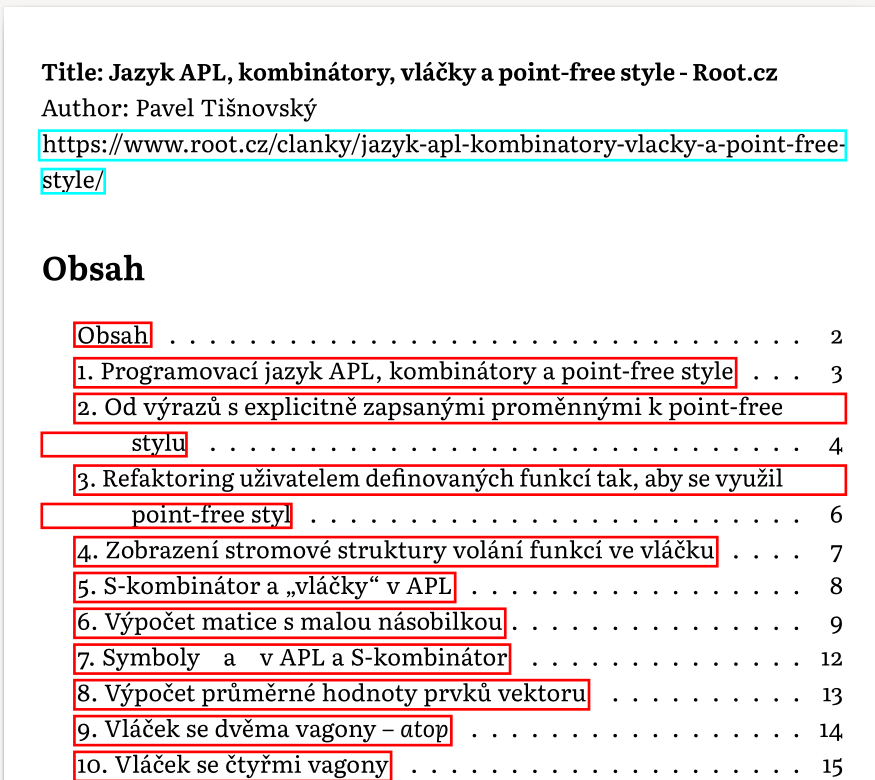
\includegraphics[height=0.7\textheight]{img/rmodepdf-article.png}
    \end{center}
    % \caption{Header of a processed page}\label{fig:rmodepdf-article}
  \end{figure}
  
\end{frame}

For each page, it displays a header with basic document information and a table
of contents. This is followed by the text of the document.



\begin{frame}[fragile]
  \frametitle{Print Transformed \LaTeX\ Code}
\begin{block}{pipe the generated TeX code to foo.tex}
\begin{verbatim}
$ rmodepdf -p <url> > foo.tex
\end{verbatim}
\end{block}
\end{frame}

If we print the page using the \verb|-p| option, the generated TeX code is output to the standard output, and no compilation occurs.



\begin{frame}[fragile]
  \frametitle{Output File Name}
  \begin{block}{save as foo.pdf}
  \begin{verbatim}
$ rmodepdf -o foo.pdf <url>
  \end{verbatim}
\end{block}
\end{frame}

The output file name is based on the first page title. If no title was detected on the page, the output file name 
is named using the following template: \verb|rmodepdf-%Y%m%d-%H-%M|. You can choose another name using 
the \verb|-o| or \verb|--output| option.

\begin{frame}[fragile]
  \frametitle{Choose Page Format and Style}
  \begin{block}{}
\begin{verbatim}
# use A4 format for the paper size 
# use plain page style
$ rmodepdf -P a4paper -s plain <url>
\end{verbatim}
\end{block}
\end{frame}


You can choose a different page size using the \texttt{-P} option. By default,
the page size and margins are set for e-book readers, but you can also select
other sizes, such as A4 paper size. The page style is currently set to empty
(\textit{blank}), but you can change it using the \texttt{-s} option.

\begin{frame}[fragile]
  \frametitle{Change Image Directory}
\begin{verbatim}
# save the document as foo.pdf and 
# save images in the temp dir
$ rmodepdf -o foo.pdf -i /tmp/img <url>
\end{verbatim}

\end{frame}


To enhance speed, images are stored in a local directory. By default, this is
the \texttt{img/} subdirectory within the current directory, but you can
specify a different directory using the \texttt{-i} option. 

\begin{frame}[fragile]
  \frametitle{Other Options}
  \begin{description}
    \item[-n] don't download images
    \item[-N] don't process \LaTeX\ math in pages
    \item[-R] don't run Rdrview
    \item[-l] debug messages log level
  \end{description}
\end{frame}


You can disable image downloading entirely with the \texttt{-n} option. 
The Rmodepdf also detects and displays \LaTeX\ mathematical commands
embedded in web pages that use MathJax or KaTeX for
rendering. This default behavior can be disabled using the \texttt{-N} option.
Additionally, the removal of page elements using Rdrview can be
disabled with the \texttt{-R} option.


\section{Configuration}

\begin{frame}[fragile]
  \frametitle{Loading of the Configuration File}
  \begin{block}{load script.lua as the configuration file}
\begin{verbatim}
$ rmodepdf -c script.lua <url>
\end{verbatim}
\end{block}
\end{frame}

Using a configuration file, we can declare custom rules for transforming HTML
to \LaTeX, change the document template, load extra packages, or modify the
processed page before transformation.


\begin{frame}[fragile]
  \frametitle{Change Settings}
\begin{verbatim}
add_to_config {
  document = {
    preamble_extras = [[
    \setmainfont{Linux Libertine O}
    ]],
  },
  img_convert = {
    -- modify the command used for 
    -- conversion of SVG images to PDF
    svg = "cairosvg -o ${dest} -",
  },
}
\end{verbatim}


\end{frame}

This example uses the command \texttt{add\_to\_config}, which safely copies new
configuration values into the original configuration. If you only want to set a
single configuration value, you can also directly write to the \texttt{config}
table:

\begin{frame}[fragile]
  \frametitle{Direct Settings}
  \begin{block}{change settings for the Geometry package}
\begin{verbatim}
config.document.geometry = "a6paper"
\end{verbatim}
\end{block}
\end{frame}

Note that settings for Geometry are automatically generated by selecting the
\verb|-p| or \verb|--pageformat| option. You can overwrite these setting using 
this variable.

\section{Callbacks}

The configuration script is executed before the actual conversion, so it cannot
directly influence the conversion process. However, we can define several
callback functions that allow us to affect the conversion. These functions are
as follows:

\begin{frame}[fragile]
  \frametitle{Available Callbacks}
  \begin{description}[\texttt{preprocess\_content}]
  \item[\texttt{preprocess\_content}] modify string with the raw HTML before
    readability and DOM parsing.
  \item[\texttt{preprocess\_dom}] modify DOM object before fetchching of images
    or handling of MathJax.
  \item[\texttt{postprocess\_dom}] modify DOM after all processing by Rmodepdf.
  \item[\texttt{postprocess}] late post-processing of the config table.
\end{description}

\end{frame}

In the following text, we will introduce some new features provided by LuaXML, 
namely DOM processing and transforming to other formats.

\begin{frame}[fragile]
  \frametitle{Example: Print the HTML Code}


\begin{verbatim}
function postprocess_dom(dom)
  print(dom:serialize())
  return dom
end
\end{verbatim}
\end{frame}

This example is useful in that it allows you to view the DOM serialized back
into HTML. You can see all the elements that were transferred from the original
HTML document after being processed by Rdrview and the functions of Rmodepdf.
It is important to return the DOM at the end of the function, this ensures that
any modifications made to the DOM are preserved and applied to the final
document.

Here's a slightly more complex example. Let's assume that Rdrview did
not remove a menu that might look like this:

\begin{frame}[fragile]
  \frametitle{Example: Remove HTML Elements}
\begin{verbatim}
<div class="menu">
... menu contents ...
</div>
\end{verbatim}
\end{frame}


We can use the \texttt{postprocess\_dom} function to remove this menu:

\begin{frame}[fragile]
  \frametitle{Example: Remove HTML Elements}
\begin{verbatim}
function postprocess_dom(dom)
  -- Find the menu using a CSS selector
  local menu = dom:query_selector(".menu")

  -- Iterate over the menu elements 
  -- and remove each one
  for _, el in ipairs(menu) do
    el:remove_node()
  end
  
  -- Return the modified DOM
  return dom
end
\end{verbatim}
\end{frame}

In this example:

\begin{enumerate}
  \item We use the \texttt{query\_selector} method to find all elements with
    the class \texttt{menu}.
  \item Iterate over each element retrieved in the previous step
    using a \texttt{for} loop.
  \item Remove each menu element using the \texttt{remove\_node} method.
  \item Return the modified DOM at the end of the function.
\end{enumerate}

This ensures that any remaining menus are removed from the final document.


% \begin{frame}
%   \frametitle{What's next?}
%   \begin{itemize}
%   \item automate the design of the output document for different display sizes
%   \item automatically prevent typesetting errors:
%     \begin{itemize}
%       \item widows and orphans
%       \item line breaks with single-letter prepositions, units, or academic titles
%       \item overflow lines when typesetting narrow columns
%     \end{itemize}
%   \end{itemize}
% \end{frame}

\begin{frame}[fragile]
  \frametitle{Other Useful LuaXML DOM Functions}
  \begin{description}[\texttt{el:get\_element\_name}]
    \item[\texttt{el:get\_attribute}] get element attribute
    \item[\texttt{el:set\_attribute}] set element text
    \item[\texttt{el:get\_text}] get text content of the element
    \item[\texttt{el:get\_element\_name}] get element name

  \end{description}

  \bigskip

  There are many more functions:
  \begin{itemize}
    \item for traversing the element tree 
    \item for creating new elements
  \end{itemize}


\end{frame}

See the LuaXML documentation for the API docs and examples of use.


\section{Transformation rules}


LuaXML allows us to create rules for transforming the DOM into various formats.
Rmodepdf includes rules for transforming basic HTML elements into \LaTeX.


\begin{frame}[fragile]

\frametitle{LuaXML DOM Tranformations}
\begin{description}[\texttt{htmlprocess.add\_custom\_action}]
  \item[\texttt{htmlprocess.add\_action}] add a new rule
  \item[\texttt{htmlprocess.add\_custom\_action}] process element using Lua
  \item[\texttt{htmlprocess.reset\_actions}] remove rules for the given selector
  \item[\texttt{\%s}] insert transformed contents of the element
  \item[\texttt{@\{<attribute name>\}}] insert value of an attribute
\end{description}
\end{frame}

In the configuration file, the variable \texttt{htmlprocess} contains an object with
rules for converting HTML elements. It provides two main functions:
\texttt{htmlprocess.reset\_actions}, which clears all rules for a given selector, and
\texttt{htmlprocess.add\_action}, which adds new rules.

A more powerful tool is the \verb|htmlprocess.add_custom_action| function, which
enables processing of elements in Lua. For an example of its usage, consult the
LuaXML documentation.

The following code displays some basic usage of the transformation library:

\begin{frame}[fragile]
  \frametitle{Rules Example}

\begin{verbatim}
htmlprocess.reset_actions("figure")
htmlprocess.reset_actions("img")
htmlprocess.add_action("img",
  [[\includegraphics[max width=\textwidth]{@{src}}]])
htmlprocess.add_action("figure", "\n\n \\noindent %s")
htmlprocess.add_action(".sample .foo", "hello: %s")
\end{verbatim}
\end{frame}

In this example, we change the default formatting for the \verb|<figure>| element and include the 
text that is contained inside using the \verb|%s| instruction. For the \verb|<img>| element, we use 
the \verb|src| attribute to get the image file name. As this element cannot contain any child elements,
we don't need to use \verb|%s| in this action. \verb|.sample .foo| is an example of using HTML class 
attributes in actions.

Using Lua's string syntax \verb|[[ ... ]]| allows for easy insertion of \LaTeX\
commands without the need for backslash doubling. When using regular quotes, as
you can see in the rule declaration for \verb|figure|, backslashes must be
doubled.

\section{Templates}

\begin{frame}[fragile]
  \frametitle{Template Basics}

\begin{itemize}
  \item Templates can access variables from the configuration.
  \item Simple custom syntax
\end{itemize}

\begin{verbatim}
# require template
$ rmodepdf -t mytemplate.tex <url>
\end{verbatim}
\end{frame}



\begin{frame}[fragile]
\frametitle{Template Syntax}
\begin{description}[Variable Printing]
  \item[Variable Printing] \verb|@{variablename}|: Prints a variable from the \verb|config| table or its sub-tables.
  
  \item[Loops] \verb|_{variablename}loop code/{separator}|: Iterates over array variables, using \verb|%s| placeholders or accessing fields directly.
  
  \item[Conditions] \verb|?{variablename}{true}{false}|: Evaluates a condition to insert content based on the presence of variables.
\end{description}

\end{frame}

\begin{frame}[fragile]
  \frametitle{Sample Template Snippet}
\begin{verbatim}
% loop over languages
\usepackage[_{document.languages}%s/{,}]{babel}
% use geometry settings
\usepackage[@{document.geometry}]{geometry}
@{document.preamble_extras}
\begin{document}
% loop over documents
_{pages}
\selectlanguage{@{language}}
% conditionaly print title
?{title}{Title: @{title}}\par}{}
% document contents
@{content}
/{\clearpage}
\end{document}
\end{verbatim}
\end{frame}

Although this example is not complete, it demonstrates the available syntax in templates.
Note that when processing an array, we must distinguish whether it contains
strings or tables. Strings are displayed using \verb|%s|. If it is a table, its
elements become active variables and can be displayed using
\verb|@{variablename}|. You can see the difference in processing the array
\verb|document.languages|, which contains languages as strings, and
\verb|pages|, which contains tables with metadata from processed pages.



\section{Responsive Design in \LaTeX}


So far, we have explored the features of Rmodepdf and LuaXML. Now, we will
focus on additional packages that can be used independently to facilitate
automated typesetting of documents.

% trick for TeX4ht to show examples as images
\ifdefined\HCode
  \long\def\fbox#1{\Picture*{}#1\EndPicture}
\fi


\begin{frame}
   \frametitle{What is Responsive Design}
   \begin{itemize}
     \item flexible structure - adjusting the size of elements on the page to the display device
     \item media queries - rules applied based on the properties of the display device (screen size, type of display, etc.)
   \end{itemize}

   Thanks to these features, the same page code can be well displayed both on a large monitor and on mobile devices.
\end{frame}

\begin{frame}
  \frametitle{Page Example on a Large Monitor}
  \begin{center}
    
\includegraphics[height=.8\textheight]{img/pedf-web-big.png}
  \end{center}
\end{frame}

\begin{frame}
  \frametitle{Page Example on a Small Screen}
  \begin{center}
    \includegraphics[height=.8\textheight]{img/pedf-web-small.png}
  \end{center}
\end{frame}

\begin{frame}
  \frametitle{The \texttt{responsive} Package}

  A package inspired by responsive design methods for web pages
  \begin{itemize}
  \item adjusting font size to match the display size
  \item sets basic document dimensions to match the new font size
  \item typographic scale for font sizes
  \item media queries
  \end{itemize}

  \bigskip

\begin{block}{Homepage}
  \url{https://ctan.org/pkg/responsive}
\end{block}
    % - changes in the number of characters per line
    % - margins using newgeometry
\end{frame}

Various sizes of spaces and other elements depend on the font size, so the
Responsive package adjusts them with each font size change to match the new
size.



\begin{frame}[fragile]
  \frametitle{Setting Font Size Based on Display Size}

  Font size can be set using the command \verb|\setsizes{number of characters per line}|.
  
\begin{columns}
  \begin{column}{0.5\textwidth}
\begin{verbatim}
\begin{minipage}{5cm}
\setsizes{25}

\lipsum[1]

\end{minipage}
\end{verbatim}
\end{column}
\begin{column}{0.5\textwidth}

\fbox{%
\begin{minipage}{5cm}
\ResponsiveSetup{lineratio=38}
\setsizes{25}

\normalsize

Lorem ipsum dolor sit amet,
consectetuer adipiscing elit.
Ut purus elit, vestibulum ut,
placerat ac, adipiscing vitae,
felis. 

\end{minipage}}
\end{column}
\end{columns}

\end{frame}

\begin{frame}[fragile]
  \frametitle{Difference in Font Size Based on Number of Characters}
\begin{columns}
  \begin{column}{0.5\textwidth}
\begin{verbatim}
\setsizes{55}
\end{verbatim}

\fbox{%
\begin{minipage}{5cm}
\setsizes{55}

\lipsum[1]

\end{minipage}}
\end{column}
\begin{column}{0.5\textwidth}
\begin{verbatim}
\setsizes{25}
\end{verbatim}

\fbox{%
\begin{minipage}{5cm}
\ResponsiveSetup{lineratio=38}
\setsizes{25}

\normalsize

Lorem ipsum dolor sit amet,
consectetuer adipiscing elit.
Ut purus elit, vestibulum ut,
placerat ac, adipiscing vitae,
felis. 

\end{minipage}}
\end{column}
\end{columns}
\end{frame}

\begin{frame}[fragile]
  \frametitle{Configuration}
  Options can be set when calling the package or later using the command \verb|\ResponsiveSetup|.

  \bigskip

  \begin{block}{Important options:}

  \begin{description}[noautomatic]
    \item[noautomatic] do not set font size automatically at the beginning of the document
    \item[characters] number of characters when automatically setting the font size
    \item[scale] typographic scale used for font sizes
    \item[lineratio] ratio used when calculating line height
  \end{description}
\end{block}

\end{frame}

When the Responsive package changes the base font size, it automatically
adjusts the sizes used for \verb|\large|, \verb|\small|, and other commands, as well as line
height and other fundamental dimensions.


\begin{frame}[fragile]
  \frametitle{Line Height}
  Line height can be influenced by the \texttt{lineratio} option. 
The higher its value, the smaller the distance between lines.

\begin{columns}
  \begin{column}{0.5\textwidth}
\begin{verbatim}
\ResponsiveSetup{lineratio=38}
\end{verbatim}

\fbox{%
\begin{minipage}{5cm}
\ResponsiveSetup{lineratio=38}
\setsizes{65}

\lipsum[1]

\end{minipage}}
\end{column}
  \begin{column}{0.5\textwidth}
\begin{verbatim}
\ResponsiveSetup{lineratio=34}
\end{verbatim}

\fbox{%
\begin{minipage}{5cm}
\ResponsiveSetup{lineratio=34}
\setsizes{65}

\lipsum[1]

\end{minipage}}
\end{column}
\end{columns}

\begin{block}{Inspired by this article:}
\url{https://www.smashingmagazine.com/2020/07/css-techniques-legibility/}
\end{block}

\end{frame}

% \newcommand\printsize[1]{\csname #1\endcsname\par\noindent Sample\par}
% \newcommand\showscale[2][.5\textwidth]{%
%       % \setsizes[38]{25}
%       \printsize{huge}
%       \printsize{LARGE}
%       \printsize{Large}
%       \printsize{large}
%       \hrule
%       \printsize{normalsize}
%       \hrule
%       \printsize{small}
%       \printsize{footnotesize}
% }

% \begin{frame}[fragile]
%   \frametitle{Font Styles}

%   The sizes of individual font styles are chosen based on the typographic scale

% \begin{columns}
%   \begin{column}{0.5\textwidth}
% Default scale (pentatonic)

% \fbox{%
% \begin{minipage}{5cm}
% \setsizes{45}

% \showscale{}

% \end{minipage}}
% \end{column}
%   \begin{column}{0.5\textwidth}
% \begin{verbatim}
% \ResponsiveSetup{scale=golden}
% \end{verbatim}

% \fbox{%
% \begin{minipage}{5cm}
% \ResponsiveSetup{scale=golden}
% \setsizes{45}

% \showscale

% \end{minipage}}
% \end{column}
% \end{columns}
% \url{https://spencermortensen.com/articles/typographic-scale/}

% \end{frame}

% \begin{frame}[fragile]
%   \frametitle{Finer Scale Adjustment}

%   We can also directly set the ratio and number of steps by which the scale increases by this ratio.

% \begin{columns}
%   \begin{column}{0.5\textwidth}
% \begin{verbatim}
% \ResponsiveSetup{ratio=2,
% number=2,scale=none}
% \end{verbatim}

% \fbox{%
% \begin{minipage}{5cm}
% \ResponsiveSetup{ratio=2,
% number=2,scale=none}
% \setsizes{45}

% \showscale{}

% \end{minipage}}
% \end{column}
%   \begin{column}{0.5\textwidth}
% \begin{verbatim}
% \ResponsiveSetup{ratio=1.3,
% number=2,scale=none}
% \end{verbatim}

% \fbox{%
% \begin{minipage}{5cm}
% \ResponsiveSetup{ratio=1.3,
% number=2,scale=none}

% \setsizes{45}

% \showscale

% \end{minipage}}
% \end{column}
% \end{columns}

% \end{frame}

\begin{frame}[fragile]
\frametitle{CSS Media Query Example}
\begin{example}{Change text color depending on the page width}
\begin{verbatim}
body {
  color: green;
}
@media screen and (max-width: 600px) {
    body {
      color: blue;
    }
}
\end{verbatim}
\end{example}
\end{frame}

This example sets a different text color for documents on screens with a maximum width of 600 pixels.


          
\begin{frame}[fragile]
  \frametitle{Media Queries in \LaTeX}
    Using the \verb|\mediaquery| command, we can test various properties:
  
    \begin{itemize}
  \item physical page size
  \item line length
  \item page orientation
\end{itemize}

Additional tests can be easily added.

\end{frame}


\begin{frame}[fragile]

  \frametitle{Media Query Example}

  This example displays fewer characters if the text width is less or equal to 4~cm.

\begin{verbatim}
\mediaquery{max-textwidth=4cm}
{\setsizes{45}}{\setsizes{60}}
\end{verbatim}
\begin{columns}
  \begin{column}{0.5\textwidth}

\fbox{%
\begin{minipage}{5cm}
\mediaquery{max-textwidth=4cm}
{\setsizes{45}}
{\setsizes{60}}

\lipsum[1]

\end{minipage}}
\end{column}
  \begin{column}{0.5\textwidth}

\fbox{%
\begin{minipage}{3.9cm}
\mediaquery{max-textwidth=4cm}
{\setsizes{45}}
{\setsizes{60}}

\lipsum[1]

\end{minipage}}
\end{column}
\end{columns}

\end{frame}

\begin{frame}
  \frametitle{Do Media Queries Make Sense in \LaTeX?}
  \begin{itemize}
    \item possibly in universal packages
    \item using different templates for different sizes is easier
  \end{itemize}
\end{frame}

\section{The \texttt{linebreaker} Package}


\newcommand\testbox[1]{%
  \parbox{150pt}{%
    \parindent=15pt%
    \tolerance=1%
    \pretolerance=1%
    #1
  }%
}

\newcommand\printtest[1]{%
  \linebreakerdisable%
  \noindent\testbox{%
    #1
    \par\medskip\noindent\hfill\textbf{Without Linebreaker}\hfill\null
  }%
  \linebreakerenable%
  \hfill%
  \testbox{%
    #1
    \par\medskip\noindent\hfill\textbf{With Linebreaker}\hfill\null
  }%
}

\begin{frame}[fragile]
  \frametitle{The \texttt{linebreaker} Package}
  Prevents the occurrence of overfull lines
  \begin{itemize}
    \item Affects only the typesetting of paragraphs where such a line occurs
    \item If it detects an overfull line in a paragraph, it retypesets it with larger values for
      \verb|tolerance| and \verb|emergencystretch|.
  \end{itemize}

  \bigskip

\begin{block}{Hopegage}
  \url{https://ctan.org/pkg/linebreaker}
\end{block}
\end{frame}

\begin{frame}
  \frametitle{Example}
  \printtest{
    The example document given below creates two pages by using Lua code alone. You
will learn how to access TeX's boxes and counters from the Lua side, shipout a
page into the PDF file, create horizontal and vertical boxes (hbox and vbox),
create new nodes and manipulate the nodes links structure. 
%The example covers the following node types: rule, whatsit, vlist, hlist and action.
  }
\end{frame}

\begin{frame}[fragile]
  \frametitle{Configuration}
  Linebreaker can be configured using the \verb|\linebreakersetup| command:

  \bigskip

  \begin{description}[maxemergencystretch]
    \item[maxcycles] number of attempts to retypeset a paragraph
    \item[maxemergencystretch] maximum value of \verb|\emergencystretch|
    \item[maxtolerance]  maximum value of \verb|tolerance|
  \end{description}

  \bigskip

\begin{block}{Example configuration:}
\begin{verbatim}
\linebreakersetup{
maxtolerance = 90,         % default 9999
maxemergencystretch = 1em, % default 3em
maxcycles = 4              % default 30
}
\end{verbatim}
\end{block}

\end{frame}

When Linebreaker detects paragraph overflow, it attempts to typeset it again
with increasing \verb|\tolerance| and \verb|\emergencystretch| values. These values are
incremented by a specified number of steps until they reach the maximum values
configured in Linebreaker. If a value is found where the paragraph no longer
overflows, processing stops, and those values are used.

\section{Conclusion}


\begin{frame}[fragile]
  \frametitle{Rmodepdf status}

  \begin{itemize}
    \item It is still work in progress, so features can change.
    \item Even if it isn't useful to you, it led to the development of the HTML parser for LuaXML, Linebreaker, and Responsive packages, each of which can be useful independently.
  \end{itemize}

\end{frame}

\begin{frame}[fragile]
  \frametitle{Other useful packages for automatic typesetting}
  \begin{description}[lua-widow-control]
    \item[lua-widow-control] prevents widows and orphans.
    \item[luavlna]  prevents single chars at end of lines for Czech and Slovak, prevents line breaks in SI units and academic titles.
  \end{description}
\end{frame}




% \section{Conclusion}

\begin{frame}[standout]
  Thank you for your attention!

  \url{michal.h21@gmail.com}

  \url{www.kodymirus.cz}
\end{frame}


